\documentclass[journal,12pt,twocolumn]{article}
\usepackage{graphicx}
\usepackage[none]{hyphenat}
\usepackage[margin=0.5in]{geometry}
\usepackage[cmex10]{amsmath}
\usepackage{array}
\usepackage{booktabs}
\usepackage{gensymb}
\usepackage{textcomp}
\title{\textbf{Line Assignment}}
\author{Dulla Srinivas - FWC22041}
\date{\today}
\providecommand{\norm}[1]{\left\lVert#1\right\rVert}
\providecommand{\abs}[1]{\left\vert#1\right\vert}
\let\vec\mathbf
\newcommand{\myvec}[1]{\ensuremath{\begin{pmatrix}#1\end{pmatrix}}}
\newcommand{\mydet}[1]{\ensuremath{\begin{vmatrix}#1\end{vmatrix}}}
\providecommand{\brak}[1]{\ensuremath{\left(#1\right)}}

\begin{document}

\maketitle
\section*{Problem Statement:}
\paragraph{The straight line 5x +4y = 0 passes through the point of
intersection of the straight lines x + 2y - 10 =0 and
2x+y+5=0. Find the point of intersection of 2 and 3 lines . and then passes 1st eqaution in 3rd equation.}

\section*{Solution:}

\begin{figure}[h]
\centering
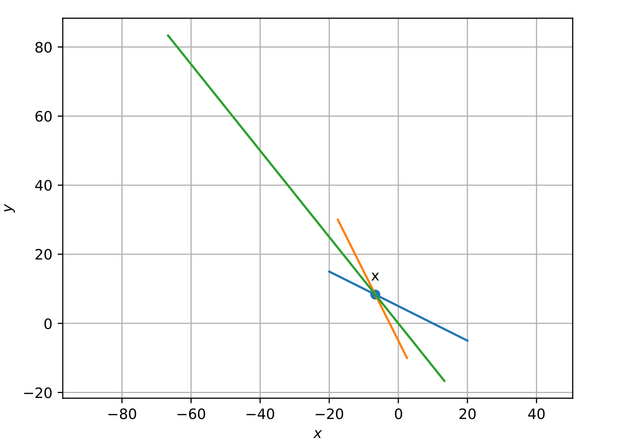
\includegraphics[width=\columnwidth]{rsz_line.png}
\caption{Diagram generated using python}
\label{fig:square}
\end{figure}
\subsection{Theory:}
They given three lines one line i.e) 5x + 4y =0 passes through the point of
intersection of the straight lines x + 2y - 10 =0 and
02x+y+5=0.}

\subsection{Mathematical Calculation:}
$\vec{O} = \myvec{0\\0}$ 
\end{center}
Given line equations are
\begin{equation}
x + 2y =10  
\end{equation}
\begin{equation}
2x+y =-5
\end{equation}

\\The parametric equation of a line  is given by  
\begin{align}
	\vec{n_1^{\top}}\vec{x}= \vec{c_1}
\end{align}\vspace{2mm}
\begin{align}
	\vec{n_2^{\top}}\vec{x}= \vec{c_2}
\end{align}\vspace{2mm}
\begin{align}
	\vec{n_3^{\top}}\vec{x}= \vec{c_3}
\end{align}\vspace{2mm}
\begin{align}   
	\myvec{\vec{n_1}\\\vec{n_2}\\\vec{n_3}}^{\top}\vec{x} &= \myvec{\vec{c_1}\\\vec{c_2}\\\vec{c_3}}
\end{align} \vspace{2mm}
The vector equation of the line x+2y-10=0  is
\begin{align}
	\vec{n_1^{\top}}\vec{x}= \vec{c_1}
\end{align}\vspace{2mm}
\begin{eqnarray}
(1\;2)\myvec{\vec{X}}=10
\end{eqnarray}
The vector equation of the line 2x+y+5=0  is
\begin{eqnarray}
\begin{align}
	\vec{n_2^{\top}}\vec{x}= \vec{c_2}
\end{align}  \vspace{2mm}
\end{eqnarray}
\begin{eqnarray}
 (2\;1)\myvec{\vec{X}}= -5
\end{eqnarray}
The vector equation of the line 5x+4y=0  is
\begin{eqnarray}
\begin{align}
	\vec{n_3^{\top}}\vec{x}= \vec{c_3}
\end{align}  \vspace{2mm}
\end{eqnarray}
\begin{eqnarray}
 (5\;4)\myvec{\vec{X}}= 0
\end{eqnarray}

The above equations can be written in matrix form as,
\center
\myvec{ 1& 2 & \\ 2 & 1 & \\ 5 & 4 &} \myvec{\vec{X} \\} = \myvec{10\\-5\\0} \\
\vspace{0.3cm}
\begin{flushleft}
The augmented matrix can be expressed as,
\end{flushleft}
\myvec{ \circled{1} & 2 & 10 \\ 2 & 1  & -5 \\ 5 & 4   & 0} \\
\begin{flushleft}
Through pivoting, the augmented matrix will become as,
\end{flushleft}
\begin{align}
			    
			    \myvec{
				    1 & 2 \vrule & 10
			    \\
			    2 & 1  \vrule & -5
			    \\
			    5 & 4 \vrule & 0}
\end{align}
\begin{align}
 \xleftrightarrow[]{R_2 \leftarrow \ R_2-2R_1}
		\myvec{
    \ 1 & 2 & \vrule & 15
			    \\
0 & -3  &\vrule & 20
\\
5 & 4  &\vrule & 0
		    }
\end{align}
\begin{align}
 			\xleftrightarrow[]{R_1 \leftarrow \ 2R_1-R_3}
			    \myvec{
				    \ 1 & 2&\vrule & 10
			    \\
			    0 & -3 &\vrule & -25
			    \\
			    5 & 4 &\vrule & 0
		    }
\end{align}

\begin{align}
  \xleftrightarrow[]{R_2 \leftarrow \ R_2-2R_1}
                \myvec{
	\ 1 & 2 & \vrule & 15
                             \\
 0 & -3  &\vrule & 20
 \\
 5 & 4  &\vrule & 0
                     }
 \end{align}



\begin{align}
 			\xleftrightarrow[]{R_3 \leftarrow \ 3R_3+5R_1}
			    \myvec{
				    \ -3 & 0&\vrule & 20
			    \\
			    0 & -3 &\vrule & -25
			    \\
			    0 & 12 &\vrule & 0
		    }
\end{align}

\begin{align}
 \xleftrightarrow[]{R_3 \leftarrow \ 4R_2+R_3}
		\myvec{
    \ -3 & 0 & \vrule & 15
			    \\
0 & -3  &\vrule & 20
\\
0 & 0  &\vrule & 0
		    }
\end{align}


\begin{flushleft}
On solving above equation the crossing point of the given equations will be,\\
\end{flushleft}
\vec{X}= \myvec{-20/3\\25/3\\0}
\endcenter
\vec{X}= \myvec{-6.8\\8.3\\0}
  \\hence the straight are passing through the concentric
  \vspace{10mm}
\section{Construction:}
The construction of given lines can be done only the x and y of given equations
\begin{table}[h]
 \centering
\setlength\extrarowheight{2pt}
 \begin{tabular}{|c|c|c|}
  \hline
  \textbf{variable} & \textbf{point} & \textbf{Description}\\
  \hline
  X & (x/y) & point of intersection \\
  
  \hline
  line1 & n_1=(1,2) c_1=(-10) & -6,8\\
  \hline                   
  line2 & n_2(2,1) c_2=(5) & -6,8\\
  \hline
  line3 & n_3=(5,4) c_3=(0)& -6,8\\
  
  \hline
 \end{tabular}
\end{table}

\end{document}
